%--------------------------------------------------------------------
%
% File: 2.SLZ.tex
% Author: Mykel Loren Brinkerhoff
% Description: Chapter on the Vowels and suprasegmentals in Santiago Laxopa Zapotec
%
%--------------------------------------------------------------------




\chapter{Vowels and suprasegmentals in Santiago Laxopa Zapotec} \label{ch:SLZ}

%-------------------------
\section{Introduction} \label{sec:SLZ-intro}
%-------------------------

Santiago Laxopa Zapotec (SLZ; \textit{Dilla'xhunh Laxup} [diʒaˀʐun lːaʂupʰ]) is a Northern Zapotec language spoken by approximately 1000 people in the municipality of Santiago Laxopa, Ixtlán,Oaxaca, Mexico and in diaspora communities throughout Mexico and the United States \citep{adlerAcousticsPhonationTypes2016,adlerDerivationVerbInitiality2018,foleyForbiddenCliticClusters2018,foleyExtendingPersonCaseConstraint2020}. 
According to \citet{smith-starkAlgunasIsoglosasZapotecas2007}, SLZ is part of the Cajonos Zapotec macro variety, which also includes Zoogocho Zapotec, Yatzachi Zapotec, Yalálag Zapotec, Tabaá Zapotec, Lachirioag Zapotec and several other varieties spoken in the Sierra Norte of Oaxaca, Mexico.

\begin{figure}[!h]
    \centering
    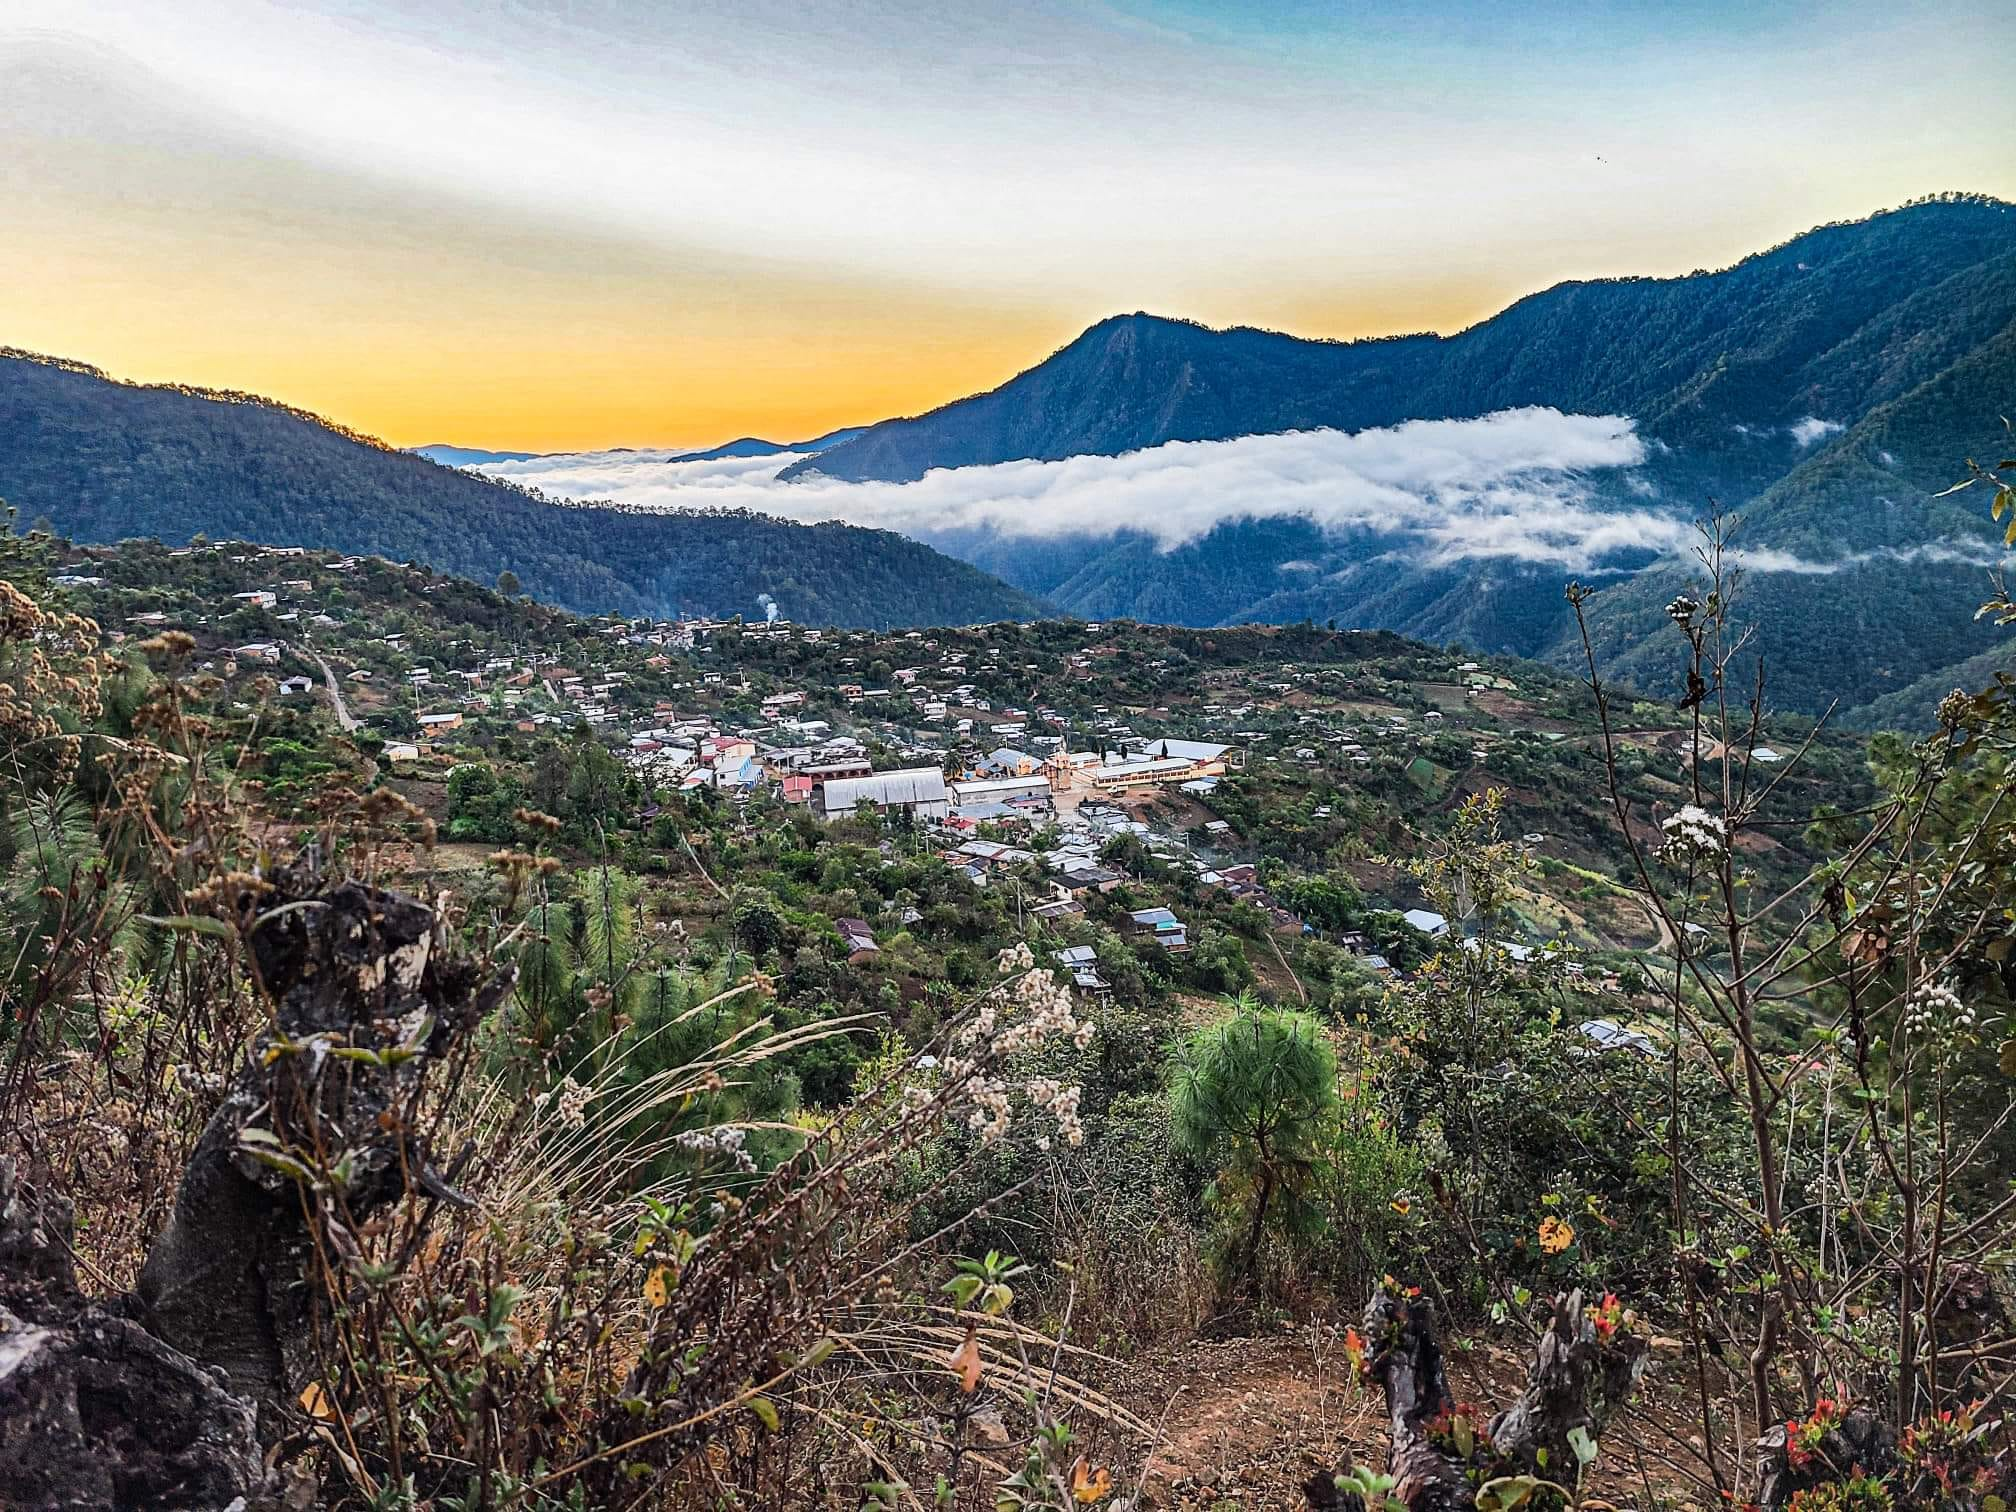
\includegraphics[width=0.9\textwidth]{Images/SantiagoLaxopa.jpeg}
    \caption{Santiago Laxopa taken by Beto Diaz, a resident of Santiago Laxopa.}
    \label{fig:SantiagoLaxopa}
\end{figure}



%-------------------------
\section{Vowels in Santiago Laxopa Zapotec} \label{sec:SLZ-vowels}
%-------------------------

SLZ exhibits a four-vowel inventory; see Table~\ref{tab:SLZvowels}. This type of vowel inventory is very common among Sierra Norte Zapotecs. Most varieties have the vowels /i/, /e/, /a/, and /o/ \citep{nellisFortisLenisCajonos1980,jaegerInitialConsonantClusters1982,butlerh.DiccionarioZapotecoYatzachi1997,avelinobecerraTopicsYalalagZapotec2004,longDiccionarioZapotecoSan2005,sonnenscheinDescriptiveGrammarSan2005}. 

\begin{table}[!h]
    \centering
    \caption{Vowel qualities in Santiago Laxopa Zapotec.}
    \label{tab:SLZvowels}
    \begin{tabular}{lccc}
        \lsptoprule
        &  front& central  & back \\
        \midrule
        high   	&  i  &     &   u$\thicksim$o \\
        mid    	&  e  &   	& 	\\
        low   	&     &  a 	&	  \\
        \lspbottomrule
    \end{tabular}
\end{table}

In SLZ the vowel /o/ is marginal in SLZ's lexicon, only appearing in a few lexical items such as the diminutive classifier \textit{do'}. This vowel is instead replaced by /u/ in most cases. This difference, however, is not universal among all speakers in the community. For the most part older speakers exhibit the vowel /o/ in their speech, while younger speakers tend to replace it with /u/. Most speakers, when asked, classify the two back rounded vowels as the same phoneme and view them as a dialectal feature between the different pueblos. For example, in neighboring San Bartolomé Zoogocho the /u/ vowel is very marginal and has led \citet{sonnenscheinDescriptiveGrammarSan2005} to describe the language as having only four vowels.It is interesting to note that everywhere that SLZ has the vowels /u/ or /o/, Zoogocho only has /o/. Further evidence for this comes from plotting the vowels along the first two formants. As shown in Figure~\ref{fig:SLZvowels}, the vowels /o/ and /u/ occupy nearly identical vowel spaces.

\begin{figure}[!h]
    \centering
    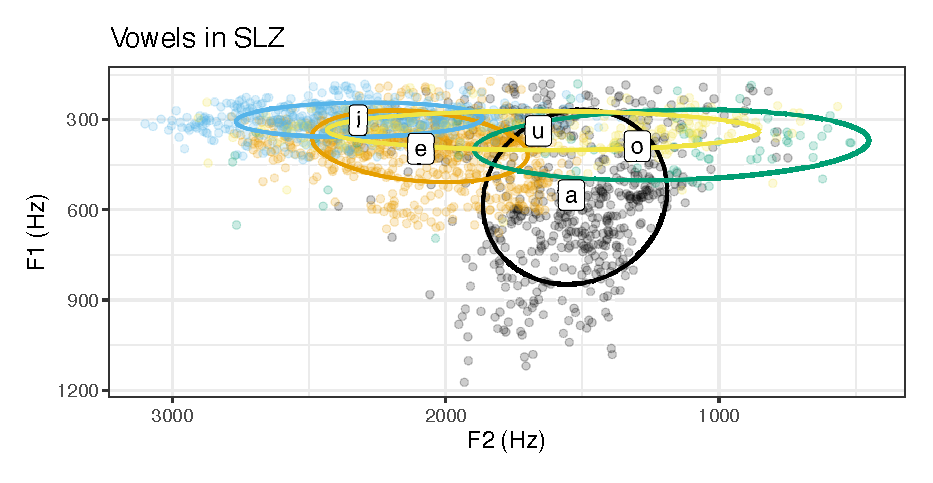
\includegraphics[width = 0.9\linewidth]{images/slz_vowels.eps}
    \caption{Vowel space of Santiago Laxopa Zapotec. The ellipses around each vowel mean represents 1 standard. The scale of the axes are in barks with their corresponding Hz values.}
    \label{fig:SLZvowels}
\end{figure}

Additional evidence for the overlap of /o/ and /u/ can be measured with a combination of Pillai scores \citep{pillaiNewTestCriteria1955,hayFactorsInfluencingSpeech2006,nyczBestPracticesMeasuring2014} and Bhattarcharyya's Affinity \citep{bhattacharyyaMeasureDivergenceTwo1943,johnsonQuantifyingOverlapBhattacharyyas2015,warrenQualityQuantityNew2018,strellufChapter3Low2018}. Both of these measures show what degree of overlap exists between two different items in some space. Their use in linguistics has primarily been used to show the process of a complete and partial mergers between vowels, such as the NEAR-SQUARE vowel merger in New Zealand English \citep{hayFactorsInfluencingSpeech2006}. The Pillai scores and Bhattacharyya's Affinity show that the vowels /o/ and /u/ are nearly identical in their vowel space; see Table~\ref{tab:SLZvowels}.

\begin{table}[!h]
    \centering
    \caption{Pillai scores and Bhattacharyya's Affinity for /o/ and /u/ in SLZ.}
    \label{tab:SLZvowels}
    \begin{tabular}{lcc}
        \lsptoprule
        &  Pillai score & Bhattacharyya's Affinity \\
        \midrule
        All speakers & 0.157 & 0.892 \\
        Females & 0.138 & 0.890 \\
        Males   & 0.224 & 0.858 \\
        \lspbottomrule
    \end{tabular}
\end{table}

In interpreting these results, Pillai scores range from 0 to 1, with 0 indicating overlap and 1 indicating complete no overlap. Bhattacharyya's Affinity ranges from 0 to 1, with 0 indicating no overlap and 1 indicating complete overlap. The results show that the overlap between /o/ and /u/ is not complete, but it is also not completely separating. This is consistent with the observations made by myself and other researchers for this variety (Toosarvandani, p.c.). 

In summary, we can conclude that SLZ is similar to other Northern Zapotec varieties in having a four-vowel inventory. The vowel /o/ is marginal in the lexicon and is often replaced by /u/ in younger speakers. The vowels /o/ and /u/ occupy nearly identical vowel spaces, and the overlap between the two vowels is not complete but is also not completely separating. 

%-------------------------
\section{Voice Quality contrasts in Santiago Laxopa Zapotec} \label{sec:SLZ-voicequality}
%-------------------------
Most Zapotec languages also make use of contrastive voice qualities (see \cite{ariza-garciaPhonationTypesTones2018} for an overview and typology of the voice quality contrasts in the Zapotec language family), with SLZ being no exception. SLZ
has a four-way voice quality contrast: modal, breathy, checked, and rearticulated. These contrasts are exemplified in the minimal quadruple in (\ref{ex:SLZphonation}).

\ea \label{ex:SLZphonation} Four-way near minimal phonation contrast
    \ea \textit{yag}  /çag\supr{L}/ `tree; wood; almúd (unit of measurement approximately 4kg)'
    \ex \textit{yah}  /ça̤\supr{L}/ `metal; rifle; bell'
    \ex \textit{yu'}  /çuˀ\supr{L}/  `cooking pot'
    \ex \textit{ya'a}  /çaˀa\supr{L}/  `market'
    \z
\z
SLZ shares with most Zpaotec varities, two types of creaky voice: checked and rearticulated. Checked vowels are characterized by an abrupt glottal closure which cuts the vowel short. This phonation is sometimes realized as a period of creakiness at the end of the vowel.

Among speakers of SLZ, there is a large amount of inter- and intra-speaker variability in how the rearticulated vowels are produced. Some speakers produce these vowels with a full glottal stop in the middle of the vowel, others produce a vowel with apparent modal voice but with a drop in amplitude (similar to what \cite{gerfenProductionPerceptionLaryngealized2005} found for some Mixtec varities), while others produce creaky voice throughout the entire vowel. Some speakers produce a combination of these unique productions. Overall, these rearticulated vowels are proiduced with some form of manipulation of glottal closure or apmlitude drop in the middle of the vowel.

[INSERT SPECTROGRAMS OF CHECKED AND REARTICULATED VOWELS]

SLZ is also unique in regards to its voice quality contrasts because it is a Northern Core Zapotec that has developed breathy voice, which has not been described in any of the neighboring Sierra Norte varieties \citep{nellisFortisLenisCajonos1980,jaegerInitialConsonantClusters1982,butlerh.DiccionarioZapotecoYatzachi1997,avelinobecerraTopicsYalalagZapotec2004,sonnenscheinDescriptiveGrammarSan2005,longDiccionarioZapotecoSan2005}.\footnote{Breathy voice in Zapotec languages, however, is common in Central Valley Zapotecs \citep{munroDiCsyonaaryTee1999,espositoSantaAnaValle2004,espositoVariationContrastivePhonation2010,uchiharaToneRegistrogenesisQuiavini2016,ariza-garciaPhonationTypesTones2018}.} Breathy voice is characterized by a raspiness throughout the whole vowel or a portion of the vowel depending on the speaker.

[INSERT SPECTROGRAM OF BREATHY VOWEL]


%-------------------------
\section{Tonal contrasts in Santiago Laxopa Zapotec} \label{sec:SLZ-tones}
%-------------------------
One of the most well known features of all Oto-Manguean languages is the fact that they are tonal languages and exhibit a large range of tonal systems \citep{pikeProblemsZapotecTone1948,renschComparativeOtomangueanPhonology1976,josserandMixtecDialectHistory1983,silvermanLaryngealComplexityOtomanguean1997,beamdeazconaProblemsZapotecTone2007,dicanioItunyosoTrique2010,dicanioCoarticulationToneGlottal2012,elliottChicahuaxtlaTriqui2016,
campbellOtomangueanHistoricalLinguistics2017a,campbellOtomangueanHistoricalLinguistics2017b,
lillehaugenOtomangueanLanguages2019,eischensTonePhonationPhonologyPhonetics2022}. SLZ has a five-way tonal contrast which consists of three level tones (high, mid, low) and two contour tones (rising and falling). 

\citet{brinkerhoffTonalPatternsTheir2022}

%------------------------------------
\section{Interactions between tone and voice quality} \label{sec:SLZ-interaction}
%------------------------------------

% Santiago Laxopa Zapotec (SLZ; \textit{Dilla'xhunh Laxup} [diʒaˀʐun laʂup]) is a Northern Zapotec language spoken by approximately 1000 people in the municipality of Santiago Laxopa, Ixtlán District in the Sierra Norte of Oaxaca, Mexico \citep{adlerAcousticsPhonationTypes2016,adlerDerivationVerbInitiality2018,foleyForbiddenCliticClusters2018,foleyExtendingPersonCaseConstraint2020}.\footnote{This macro variety is also sometimes called Cajonos Zapotec and comprises the dialects of Zoogocho Zapotec, Yatzachi Zapotec, Yalálag Zapotec, Tabaá Zapotec, and Lachirioag Zapotec \citep{smith-starkAlgunasIsoglosasZapotecas2003}.} It is mutually intelligible with San Bartolomé Zoogocho Zapotec \citep{longDiccionarioZapotecoSan2005,sonnenscheinDescriptiveGrammarSan2005}. SLZ has a fairly standard five-vowel inventory; see Table~\ref{tab:SLZvowels}.\footnote{The /o/ vowel is marginal in the lexicon for SLZ and only appears in a few lexical items. In neighboring San Bartolomé Zoogocho the /u/ vowel is very marginal and has led \citet{sonnenscheinDescriptiveGrammarSan2005} to describe the language as having only four vowels. It is interesting to note that everywhere that SLZ has the vowels /u/ or /o/, Zoogocho only has /o/. When plotting the vowel spaces and looking for outliers in the data based on F1 and F2, I noticed that the vowels /o/ and /u/ occupy nearly identical vowel spaces.}


		
% Among Zapotecan languages, it is quite common for languages to make use of contrastive phonation \citep[e.g.,][]{avelinobecerraTopicsYalalagZapotec2004,longDiccionarioZapotecoSan2005,avelinoAcousticElectroglottographicAnalyses2010,lopeznicolasEstudiosFonologiaGramatica2016,chavez-peonInteractionMetricalStructure2010}. In \posscitet{ariza-garciaPhonationTypesTones2018} typological description of phonation in Zapotecan languages, most have two to three phonation types which are described as involving creaky phonation or a glottal closure that is considered a vocalic feature. \citet{ariza-garciaPhonationTypesTones2018} additionally notes that breathy phonation is quite rare among Zapotecan languages, with only three languages in her typological study having this phonation type. Based on this typological data, she claims that breathy phonation is a recent innovation and is restricted to the Valley Zapotec languages only. However, SLZ, as a Northern Zapotec language, presents evidence to the contrary. SLZ has a four-way phonation contrast: modal, breathy, checked, and laryngealized. These contrasts are exemplified in the minimal quadruple in (\ref{ex:YA}).
% \ea \label{ex:YA} Four-way near minimal phonation contrast
%     \ea \textit{yag}  /çag\supr{L}/ `tree; wood; almúd (unit of measurement approximately 4kg)'
%     \ex \textit{yah}  /ça̤\supr{L}/ `metal; rifle; bell'
%     \ex \textit{yu'}  /çuˀ\supr{L}/  `earth'
%     \ex \textit{ya'a}  /çaˀa\supr{L}/  `market'
%     \z 
% \z 

% In representing the checked and laryngealized vowels, I follow the same procedure as other authors (e.g., \citet{avelinoAcousticElectroglottographicAnalyses2010, uchiharaToneRegistrogenesisQuiavini2016}) in representing the ``glottal stop'' element as a superscript glottal stop in the IPA transcription (i.e., [aˀ] or [aˀa]). This is primarily done as a way of standardizing the variable pronunciation of the glottal element in Zapotec, ranging from a full glottal stop (i.e., [aʔ] or [aʔa]) to a creaky portion of the vowel (i.e., [aa̰] or [aa̰a ]).  
% Theoretically, one could argue that checked and laryngealized vowels are not actually phonation types but involve a glottal stop consonant, either as a syllabic onset or coda. It is indeed logical that this could be the case. However, much work has shown that this cannot be true in Zapotec for the laryngealized vowels, which have a glottal closure in their center. \citet{chavez-peonInteractionMetricalStructure2010} summarizes this work and offers six reasons why these ``glottal stops" are a vocalic feature, not a consonant in laryngealized vowels. The first reason has to do with the distribution of the glottal stop. If it is indeed a coda or onset, then we would expect it could also occur word-initially or in consonant clusters. This does not happen in SLZ or other Zapotec languages \citep{jaegerInitialConsonantClusters1982}. Another point that he raises is that when linguists ask native language consultants about how many syllables or beats the word has, they treat laryngealized vowels as if they only had a single beat.\footnote{This is something Maya Wax Cavallaro and I tested with one of our consultants. The only times that they said one of these laryngealized vowels was not a single beat was when they had differing vowel qualities on either side of the glottal closure (e.g., \textit{bi'a} [biˀa] `fly (insect)').} These and other points raised by \citeauthor{chavez-peonInteractionMetricalStructure2010} are presented in (2). 

% \ea  Summary: glottal stop as a vocalic feature in laryngealized vowels (adapted from \cite{chavez-peonInteractionMetricalStructure2010}).
%     \ea /ʔ/ defective distribution (not in onset, not in clusters)
%     \ex Larynealized vowels have the same tonal sequences as single vowels
%     \ex Monosyllabic tendency of the majority of languages (roots = 1σ)
%     \ex *VʔC\sub{fortis}, predicted by bimoraicity of laryngealized vowels
%     \ex Same vowel quality, i.e., one vowel gesture (diphthongs a minority)
%     \ex Perceived as single syllables by native speakers (ʔ ≠ sufficient consonantal barrier, i.e., syllable boundary)
%     \z 
% \z 

% One point that he doesn't mention is that if we assume the glottal stop is a coda consonant, then we would also expect to see the other phonation types being able to co-occur with this coda consonant. Much work still needs to be done from a phonological perspective. Treating /ʔ/ and /h/ as a vocalic feature or as a consonant is worth further study, but in the present work, I assume these sounds are vocalic features and contribute to the phonation contrasts following the traditional interpretation of these sounds. 

% Breathy vowels in SLZ are characterized by a raspiness throughout the whole vowel or a portion of the vowel; see Figure~\ref{fig:BreathyVowel}. For some speakers, it appears as if the breathiness is aligned with the beginning of the vowel and others have it aligned to the end of the vowel. 

% \begin{figure}[!h]
% 	\centering
% 	% [INSERT YAH SPECTROGRAM AND WAVEFORM]
% 	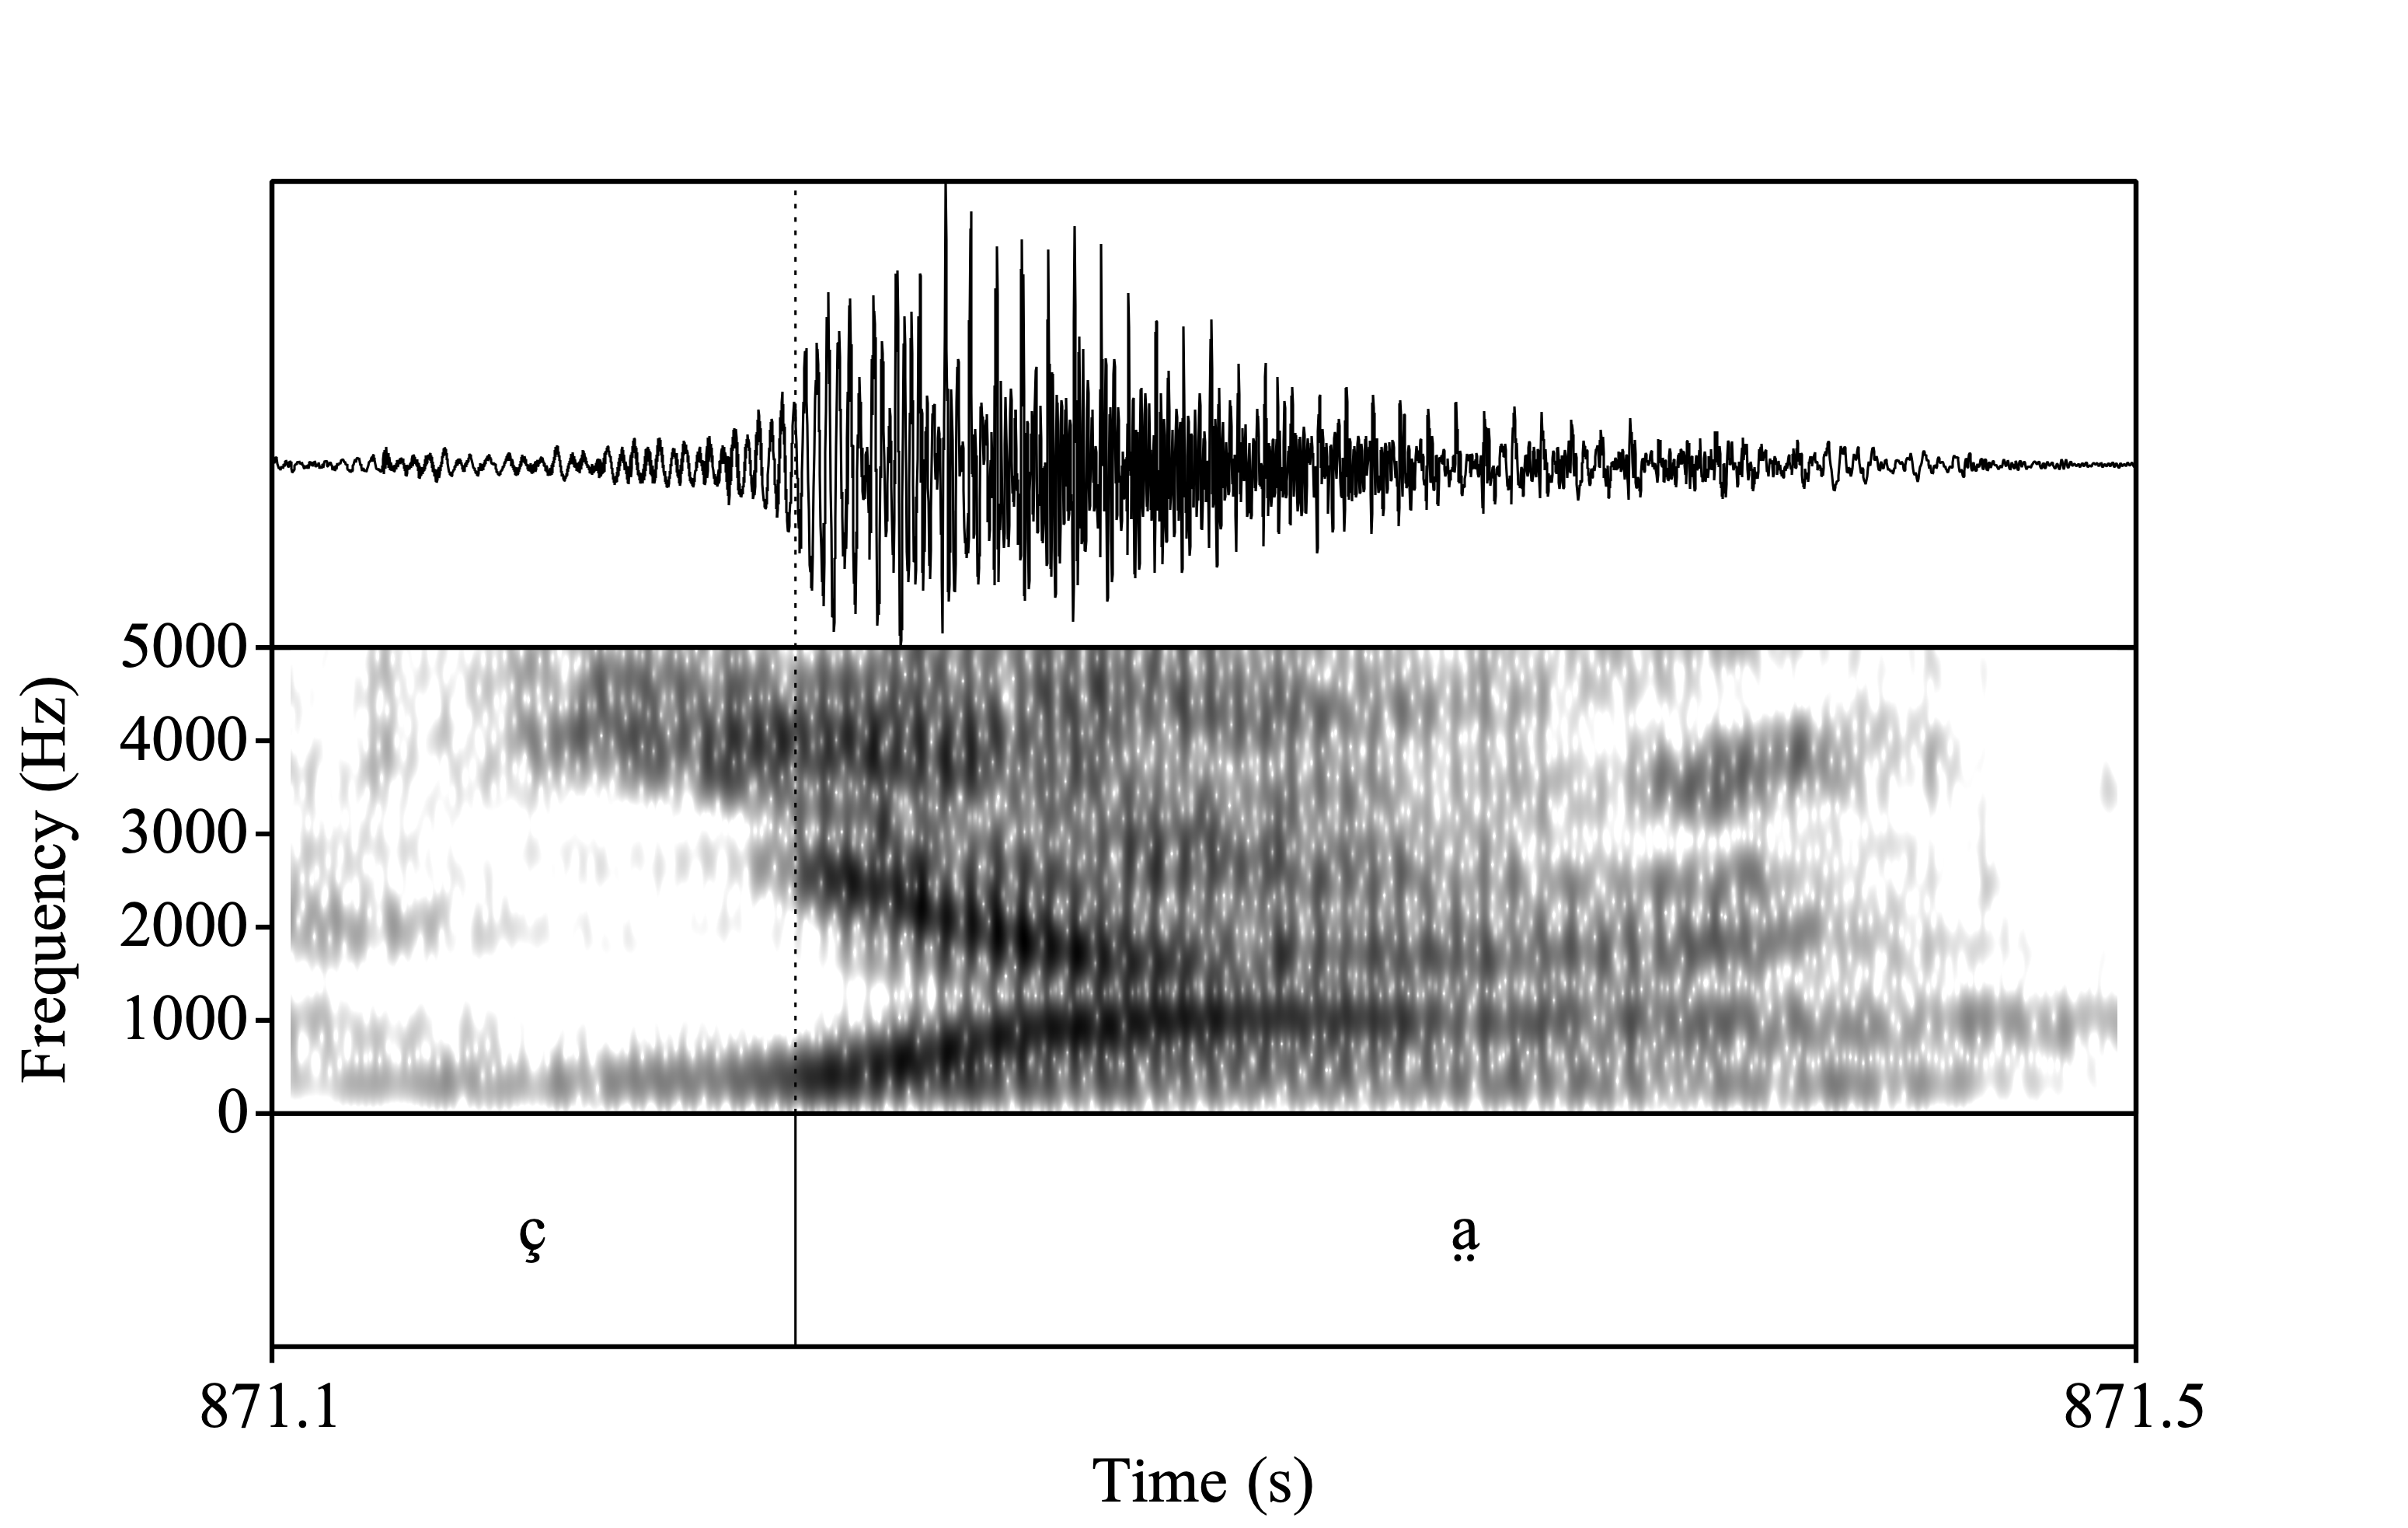
\includegraphics[width=0.9\textwidth]{Images/yah.png}
% 	\caption{Breathy vowel in the word \textit{yah} `metal; rifle'}
% 	\label{fig:BreathyVowel}
% \end{figure}

% On the other hand, checked vowels are characterized by an abrupt glottal closure which cuts the vowel short. This phonation is sometimes realized as a period of creakiness at the end of the vowel; see Figure~\ref{fig:CheckedVowel}.  

% \begin{figure}[!h]
% 	\centering
% 	% [INSERT YA SPECTROGRAM AND WAVEFORM]
% 	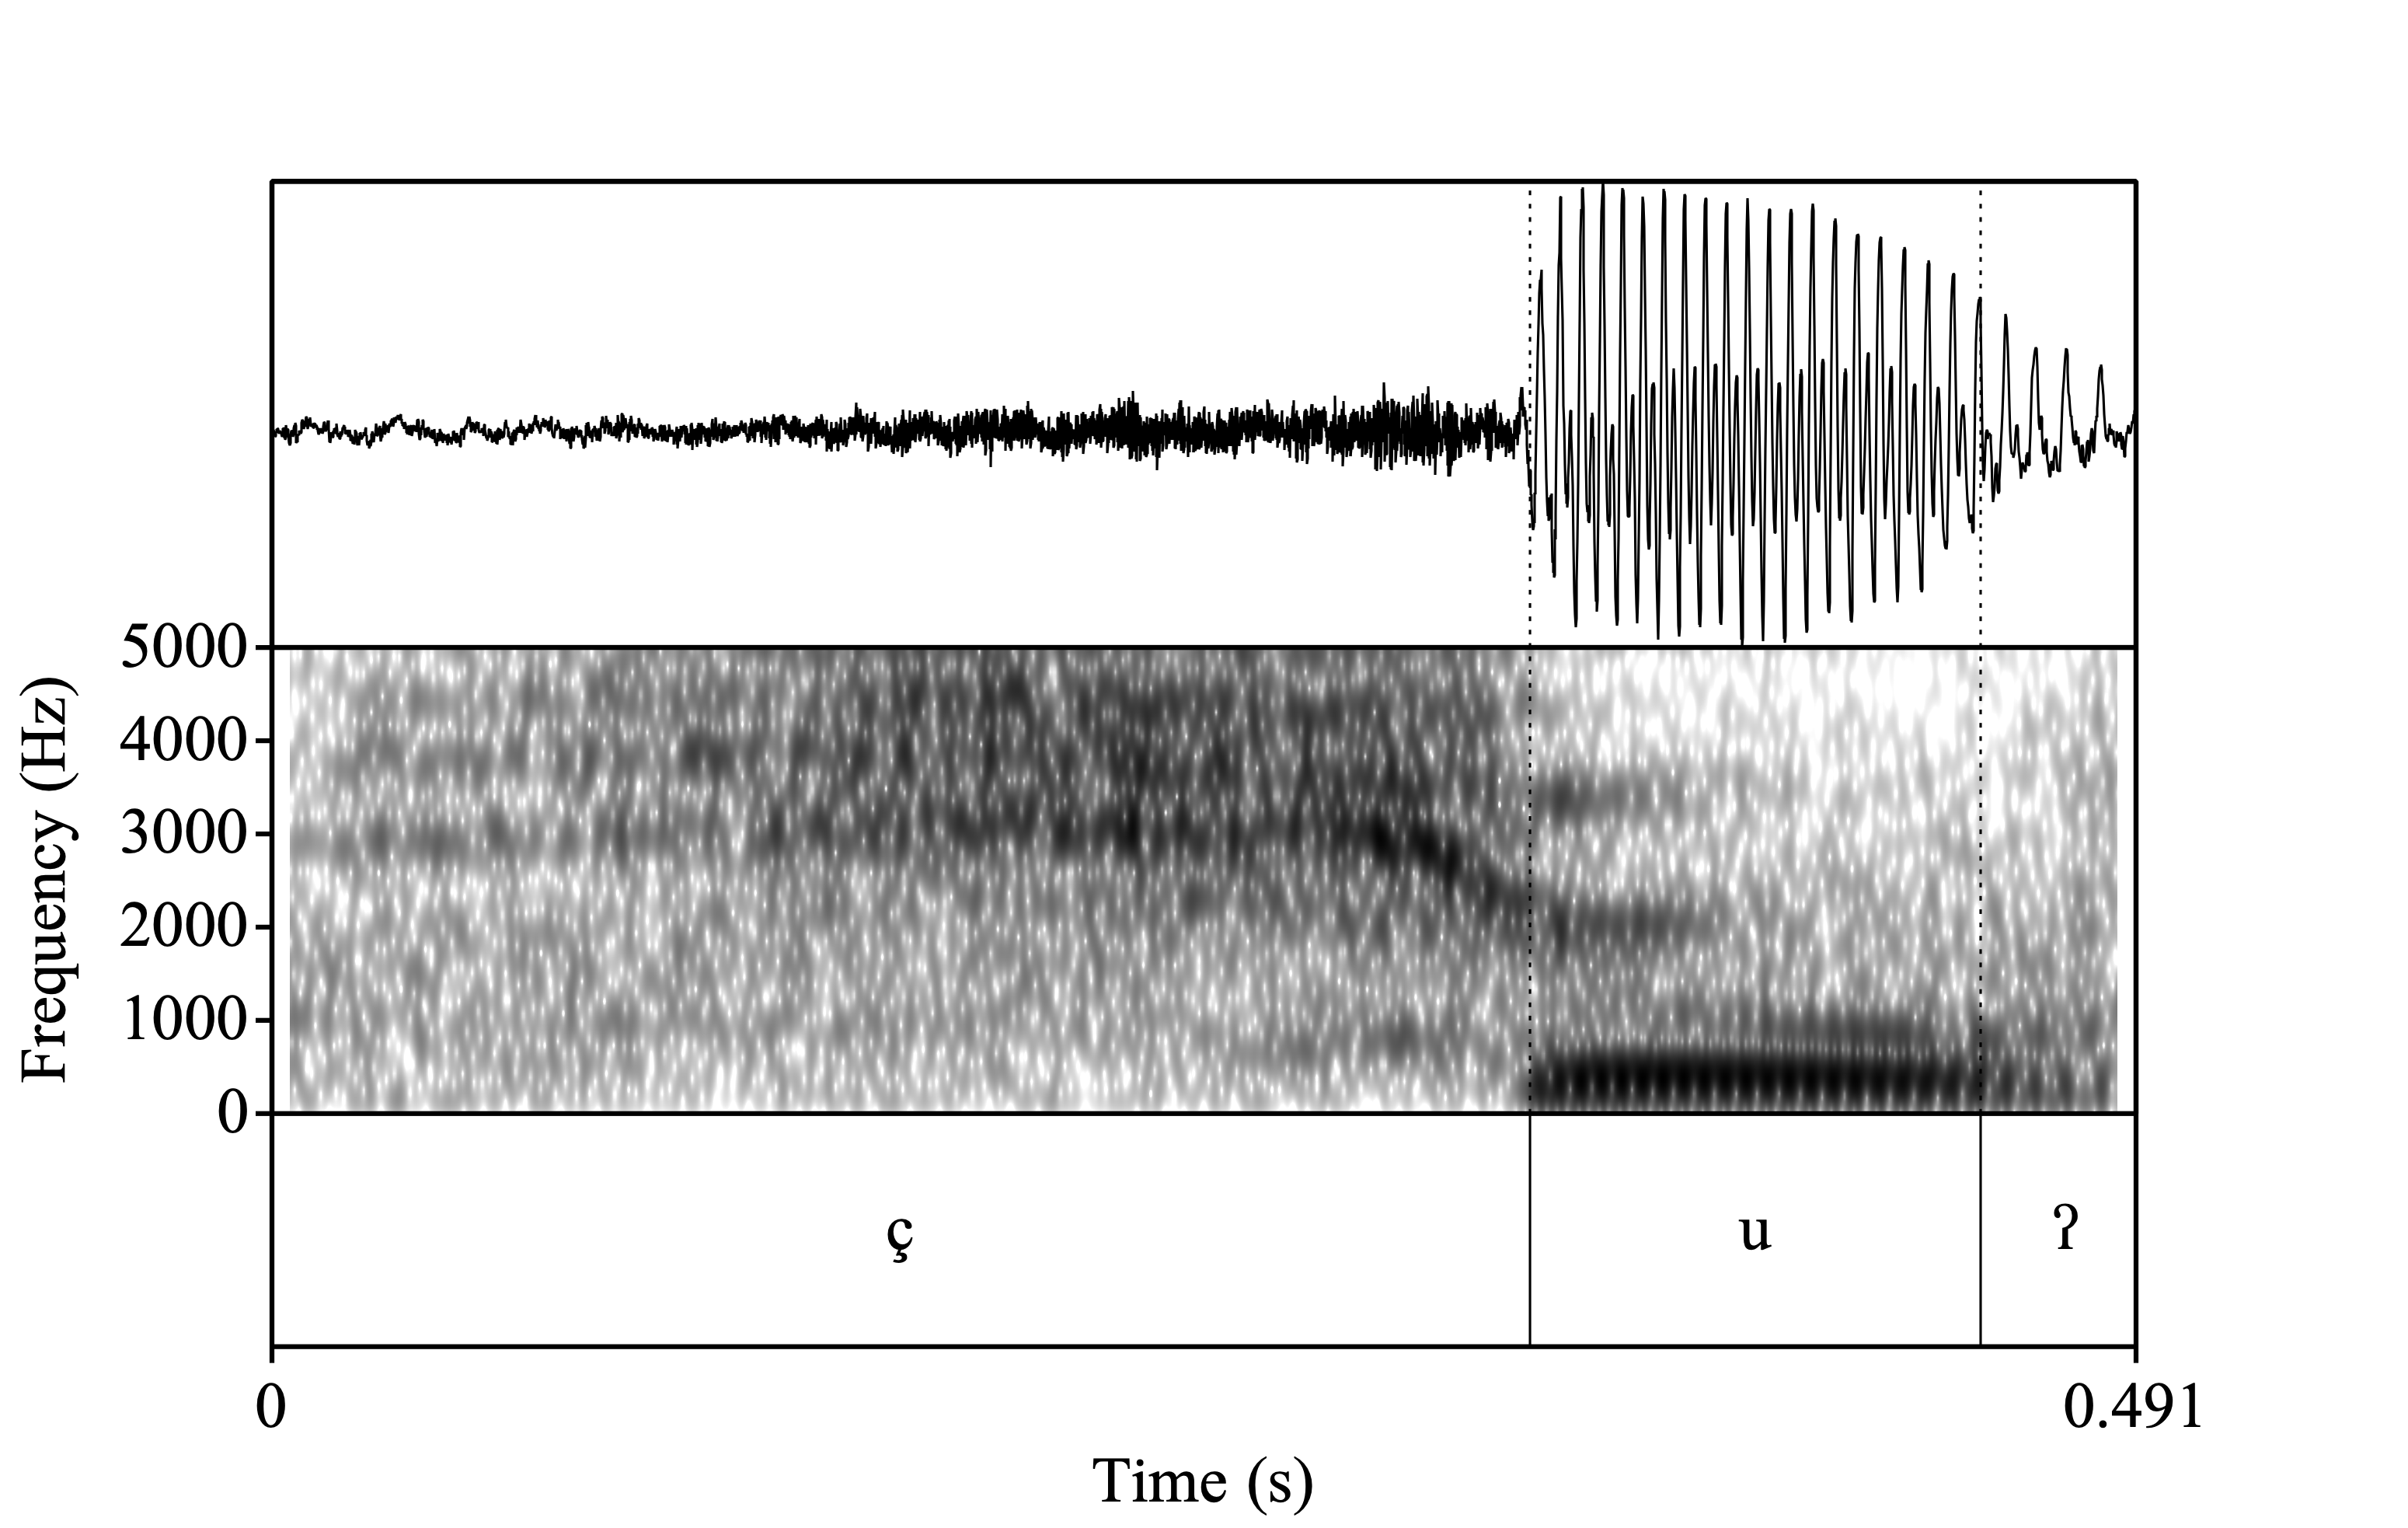
\includegraphics[width=0.9\textwidth]{Images/RD_yu'.png}
% 	\caption{Checked vowel in the word \textit{yu'} `earth'}
% 	\label{fig:CheckedVowel}
% \end{figure}

% Laryngealized vowels are common in Zapotecan languages and have received many names. Previous descriptions have used terms such as broken, rearticulated, interrupted, and creaky to describe this phonation type \citep{longDiccionarioZapotecoSan2005,avelinobecerraTopicsYalalagZapotec2004,avelinoAcousticElectroglottographicAnalyses2010,sonnenscheinDescriptiveGrammarSan2005,adlerAcousticsPhonationTypes2016}. To avoid confusion; I will use the term laryngealized following \citet{avelinoAcousticElectroglottographicAnalyses2010}. In addition to their many different names, these vowels exhibit a wide range of allophones. 

% \citet{avelinoAcousticElectroglottographicAnalyses2010} found in the closely related Yalálag Zapotec that among his consultants, there were at least four different pronunciations as seen in Table~\ref{tab:laryngeal}. 
% \begin{table}[!h]
% 	\centering
% 	\caption{Layngealized Vowels in Yalálag Zapotec}
% 	\label{tab:laryngeal}
% 	 \begin{tabular}{ll}
% 	\lsptoprule
% 	/VˀV/	&  [VʔV]  \\
% 			&  [VV̰V]   \\
% 			&  [VV̰ːV̆]  \\
% 			&  [VV̰V̰]	\\
% 	\lspbottomrule
% 	\end{tabular}
% \end{table}

% In SLZ, this vowel is also highly variable. For most speakers, laryngealized vowels were either creaky throughout their entire production or had a period of creakiness in the middle of the vowel. However, there is a large amount of inter- and intra-speaker variability in how this sound is produced. Some of these other productions included producing modal voice throughout, except for a short period of two or three glottal pulses, which showed a drop in amplitude of five to ten decibels. This drop in amplitude is not too surprising as \citet{gerfenProductionPerceptionLaryngealized2005} showed that this drop in amplitude was sufficient to cue these laryngealized vowels in Coatzospan Mixtec, a member of the Amuzgo-Mixtecan branch of the Oto-Manguean language family. Another frequent production was a complete glottal closure in the middle of the vowel producing a true re-articulation of the vowel. In addition to these productions, combinations of these unique productions were also encountered. Based on my observations, these differences cannot be attributed to sociolinguistic factors (e.g., age, sex, gender, socio-economic status) but seem to be in free variation. 

% To showcase some of these production differences, I show the production of two SLZ speakers who live in Santa Cruz, CA, who participated in piloting this study before I went to Santiago Laxopa for data collection. One of the SLZ speakers in Santa Cruz would re-articulate with a full glottal stop in the middle of the vowel or produce creaky voice. This alternation seemed to be in free variation. Still, there was a greater tendency to creak in low-toned words, such as \textit{xa'ag} [ʂa̰ːg] `topil'\footnote{A \textit{topil} is a type of government office in traditional Oaxacan communities somewhat akin to a sheriff.}, and re-articulate elsewhere; see Figure~\ref{fig:FSRLaryngeal}.

% \begin{figure}[!h]
% 	\centering
% 	\begin{subfigure}{.5\textwidth}
% 		\centering
% 		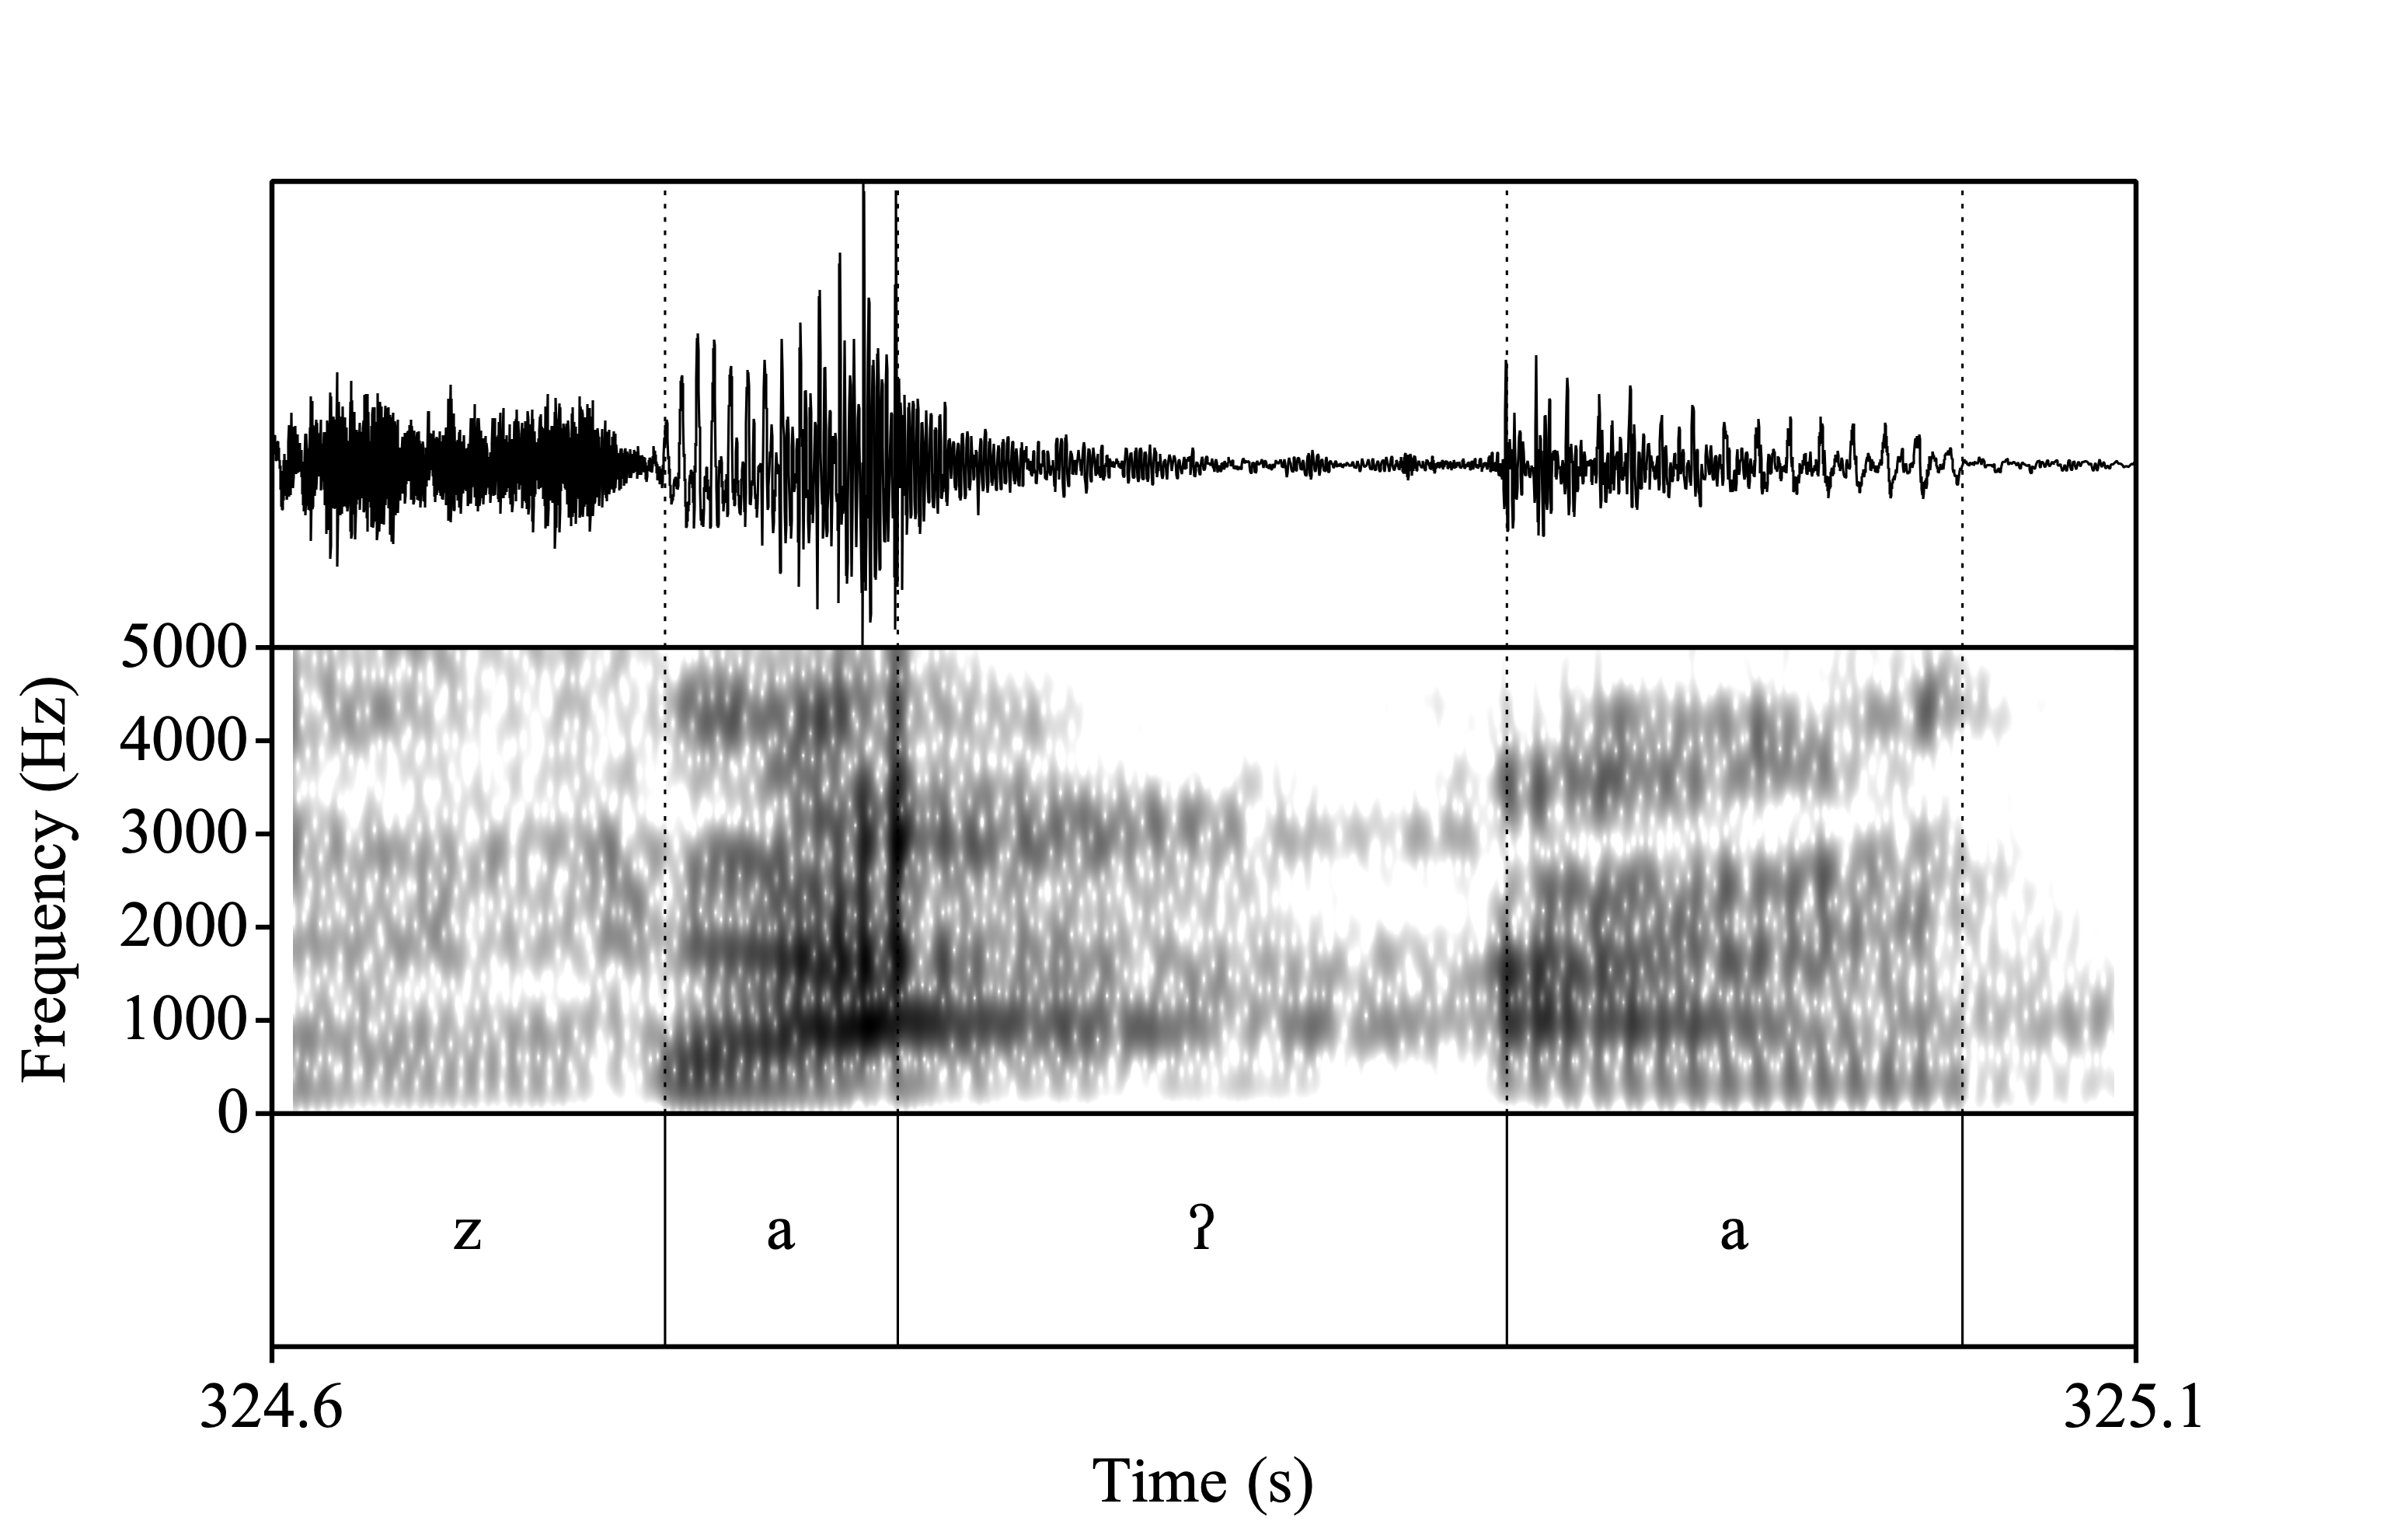
\includegraphics[width=\linewidth]{Images/za'a.png}
% 		\caption{\textit{za'a} `corncob'}
% 		\label{fig:FSRza'a}
% 	\end{subfigure}%
% 	\begin{subfigure}{.5\textwidth}
% 		\centering
% 		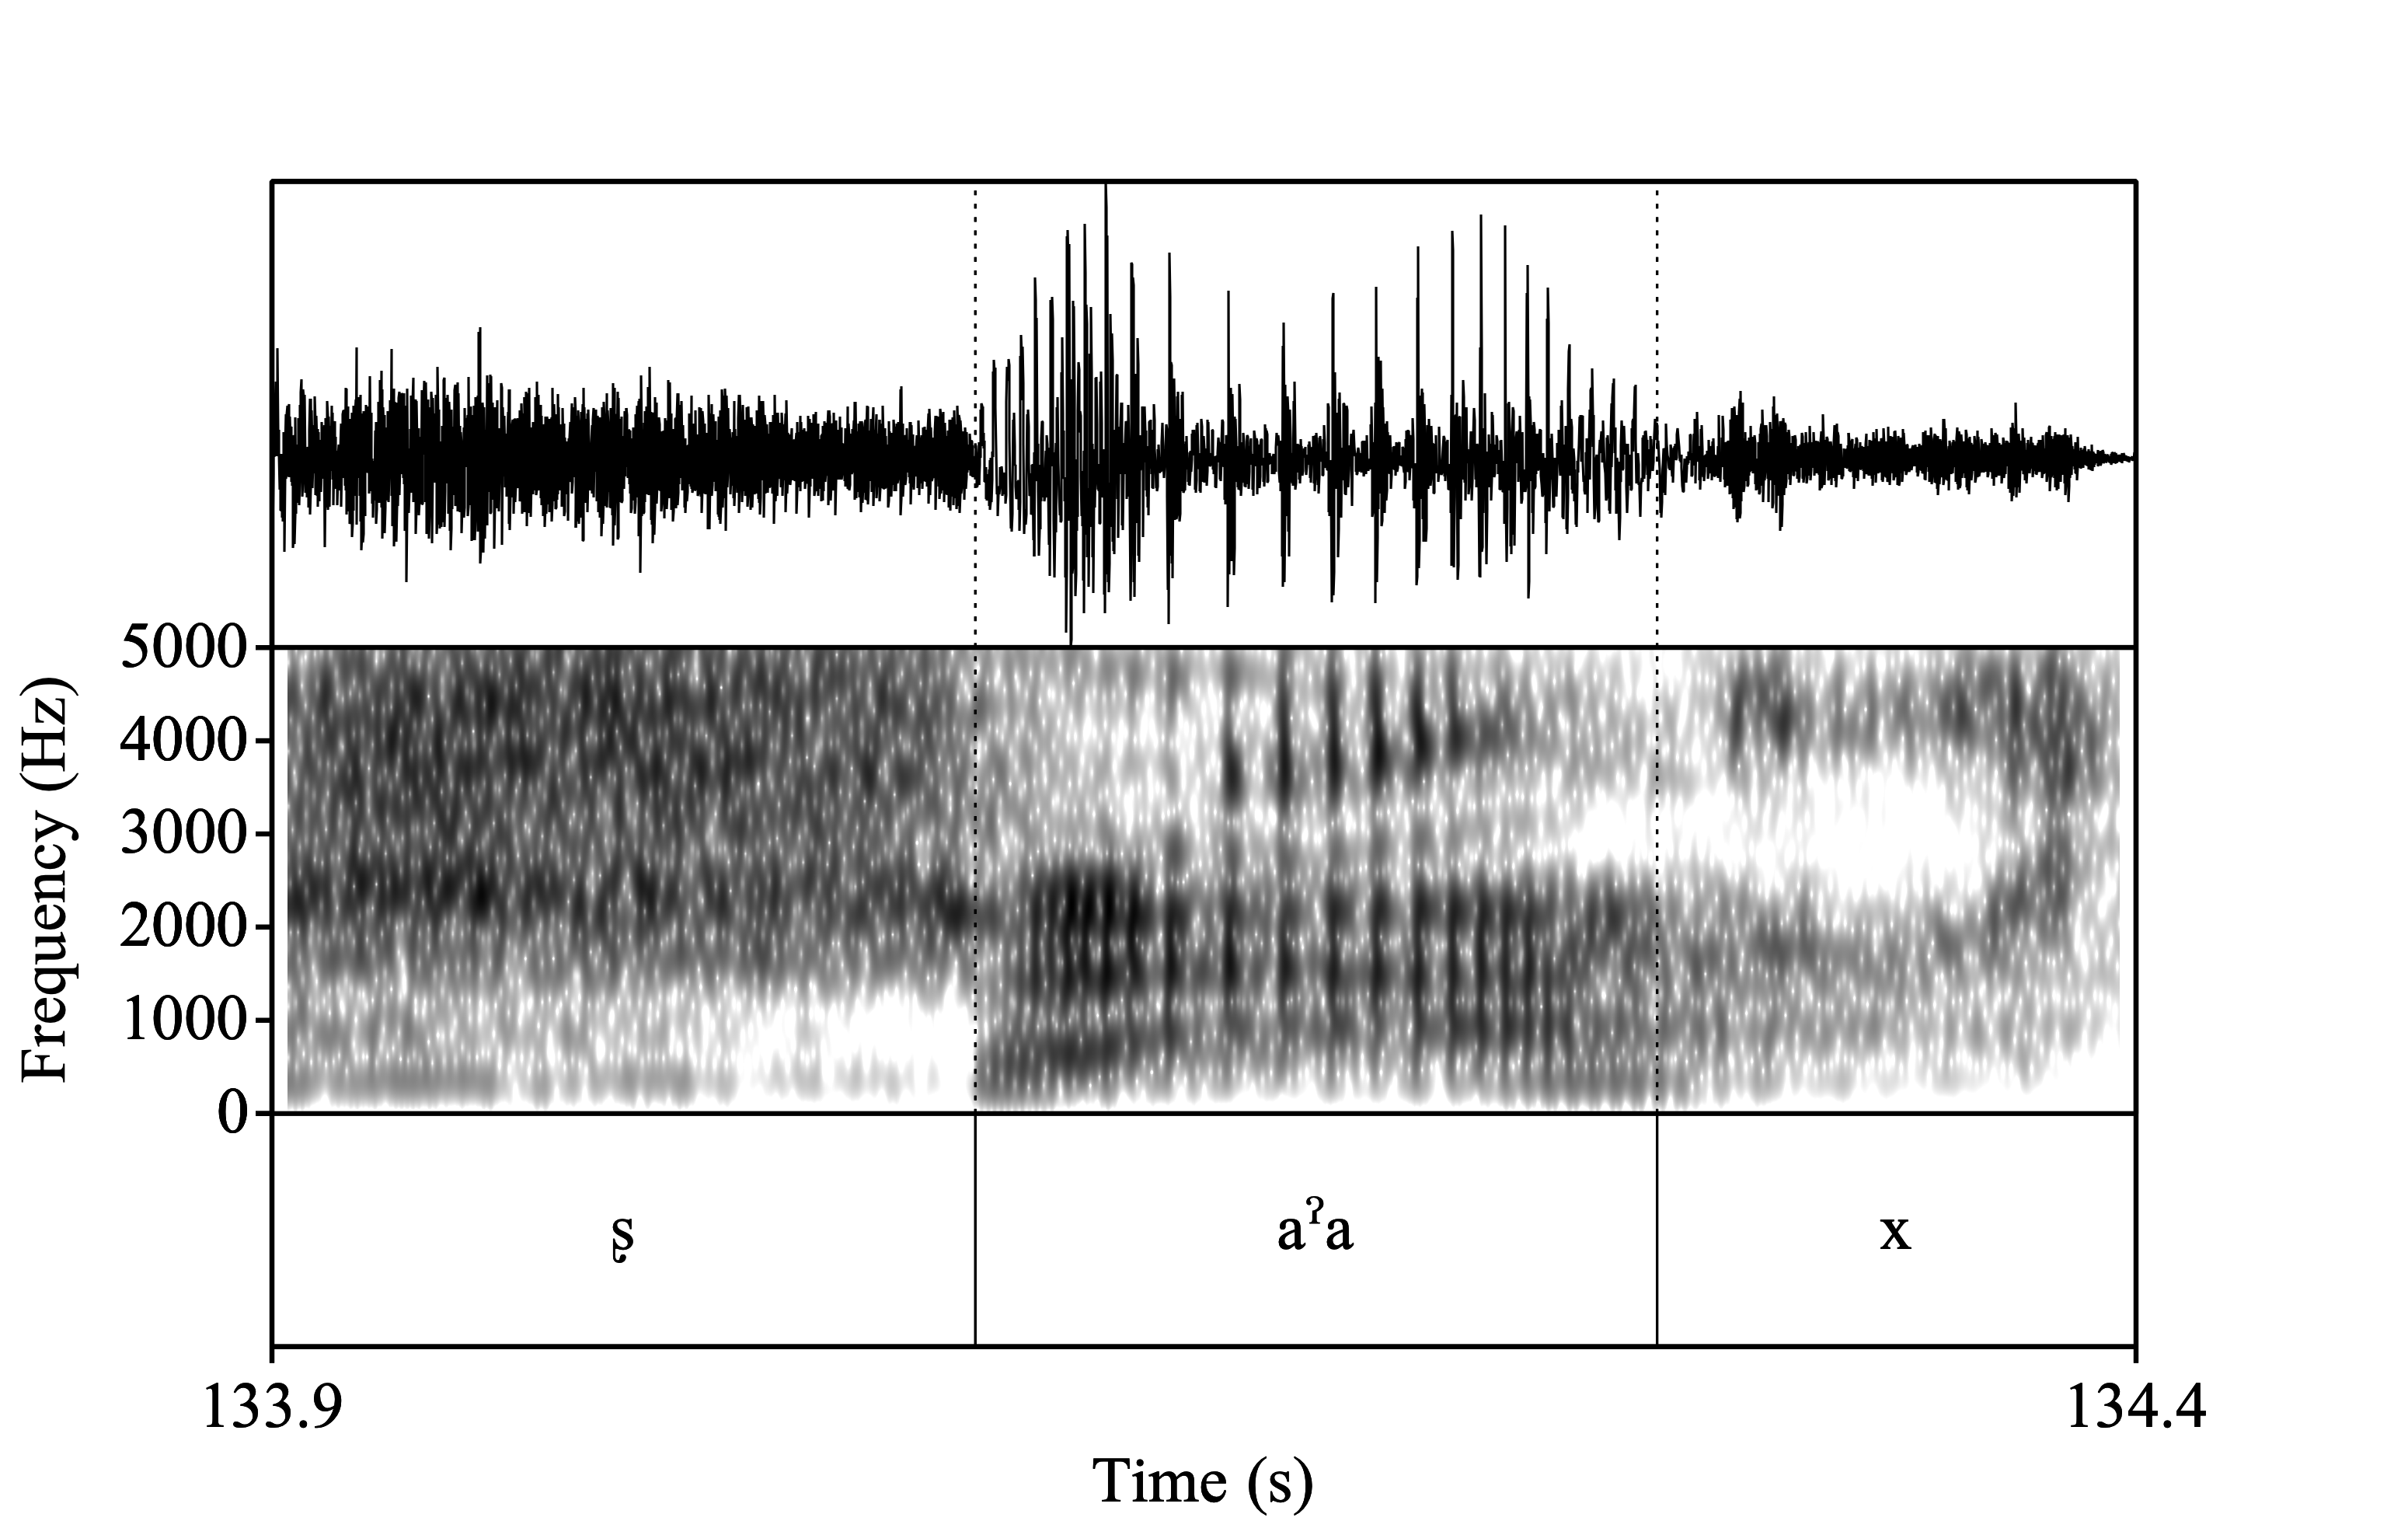
\includegraphics[width=\linewidth]{Images/xa'ag.png}
% 		\caption{\textit{xa'ag} `topil'}
% 		\label{fig:FSRxa'ag}
% 	\end{subfigure}	
% 	\caption{Comparison of FSR's laryngealized vowels in \textit{za'a} `corncob' and \textit{xa'ag} `topil'}
% 	\label{fig:FSRLaryngeal}
% \end{figure}

% The other SLZ speaker only produces creaky voice for these vowels regardless of the tone of the word. During one of the elicitation sessions, my fellow researchers and I conducted a perceptual check that these were, in fact, the same vowels. Both consultants reliably identified the words. They produced laryngealized vowels according to their own idiosyncrasies.
% \begin{figure}[!h]
% 	\centering
% 	\begin{subfigure}{.5\textwidth}
% 		\centering
% 		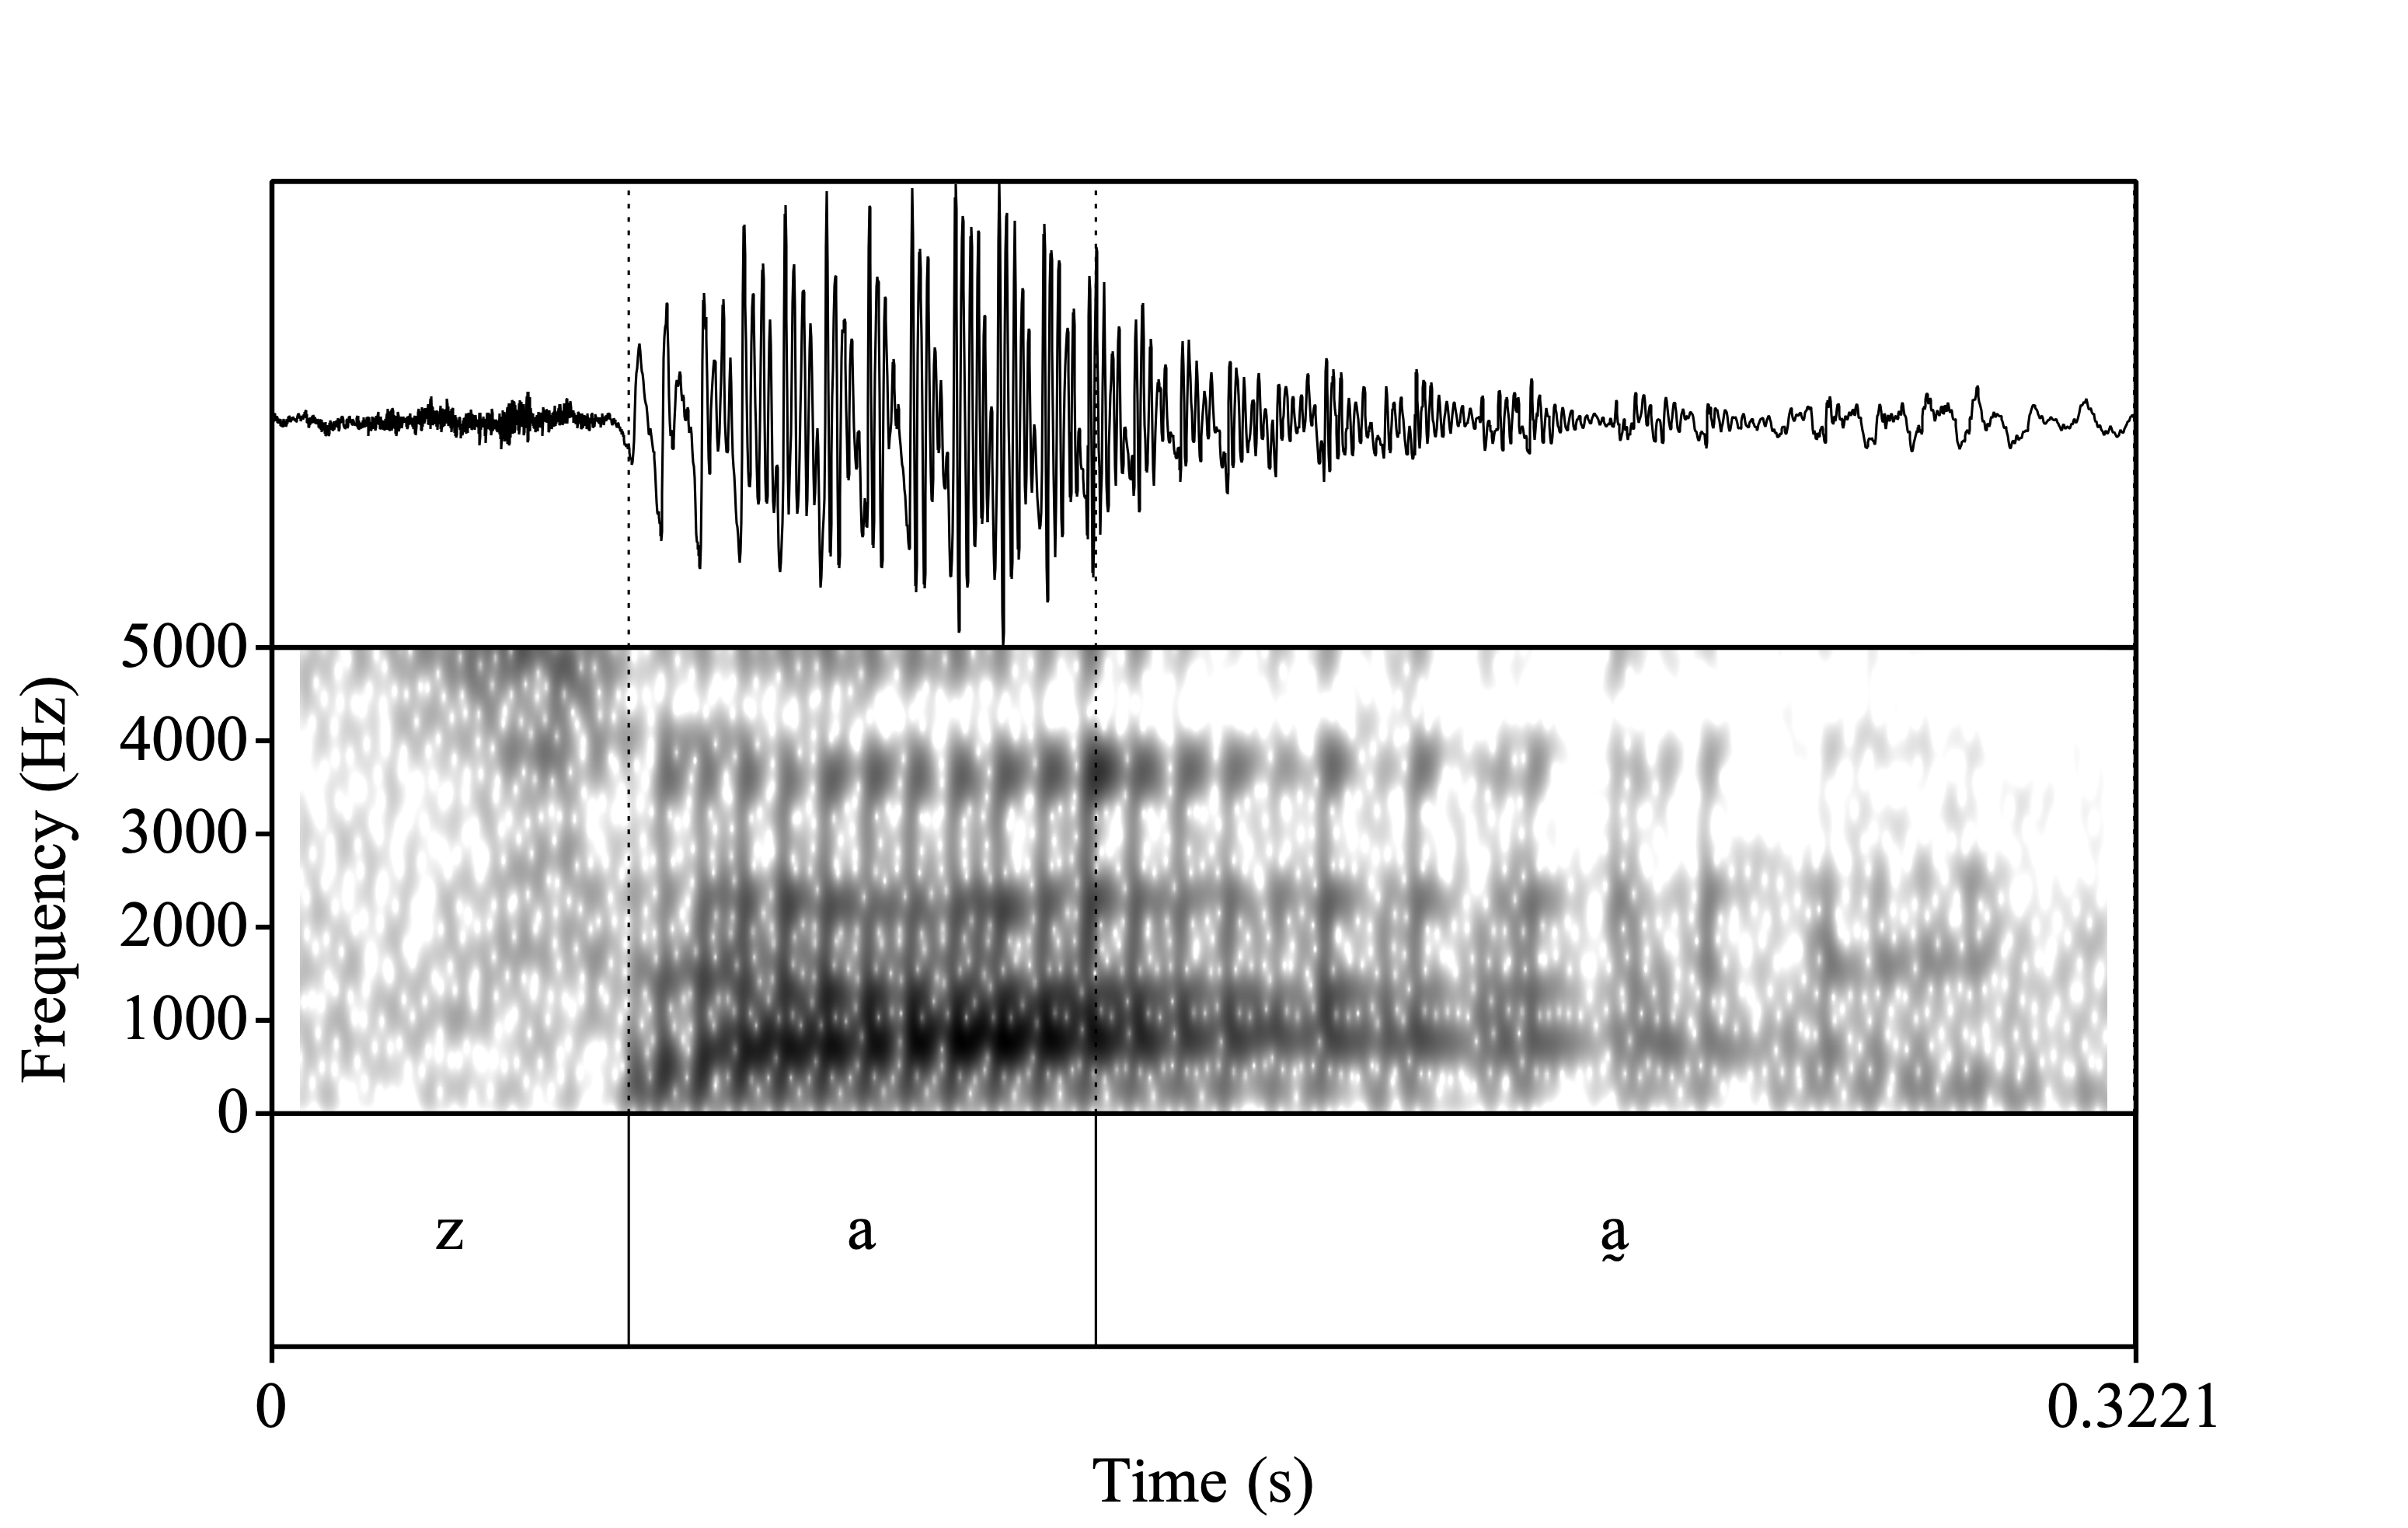
\includegraphics[width=\linewidth]{Images/RD_za'a.png}
% 		\caption{\textit{za'a} `corncob'}
% 		\label{fig:RDza'a}
% 	\end{subfigure}%
% 	\begin{subfigure}{.5\textwidth}
% 		\centering
% 		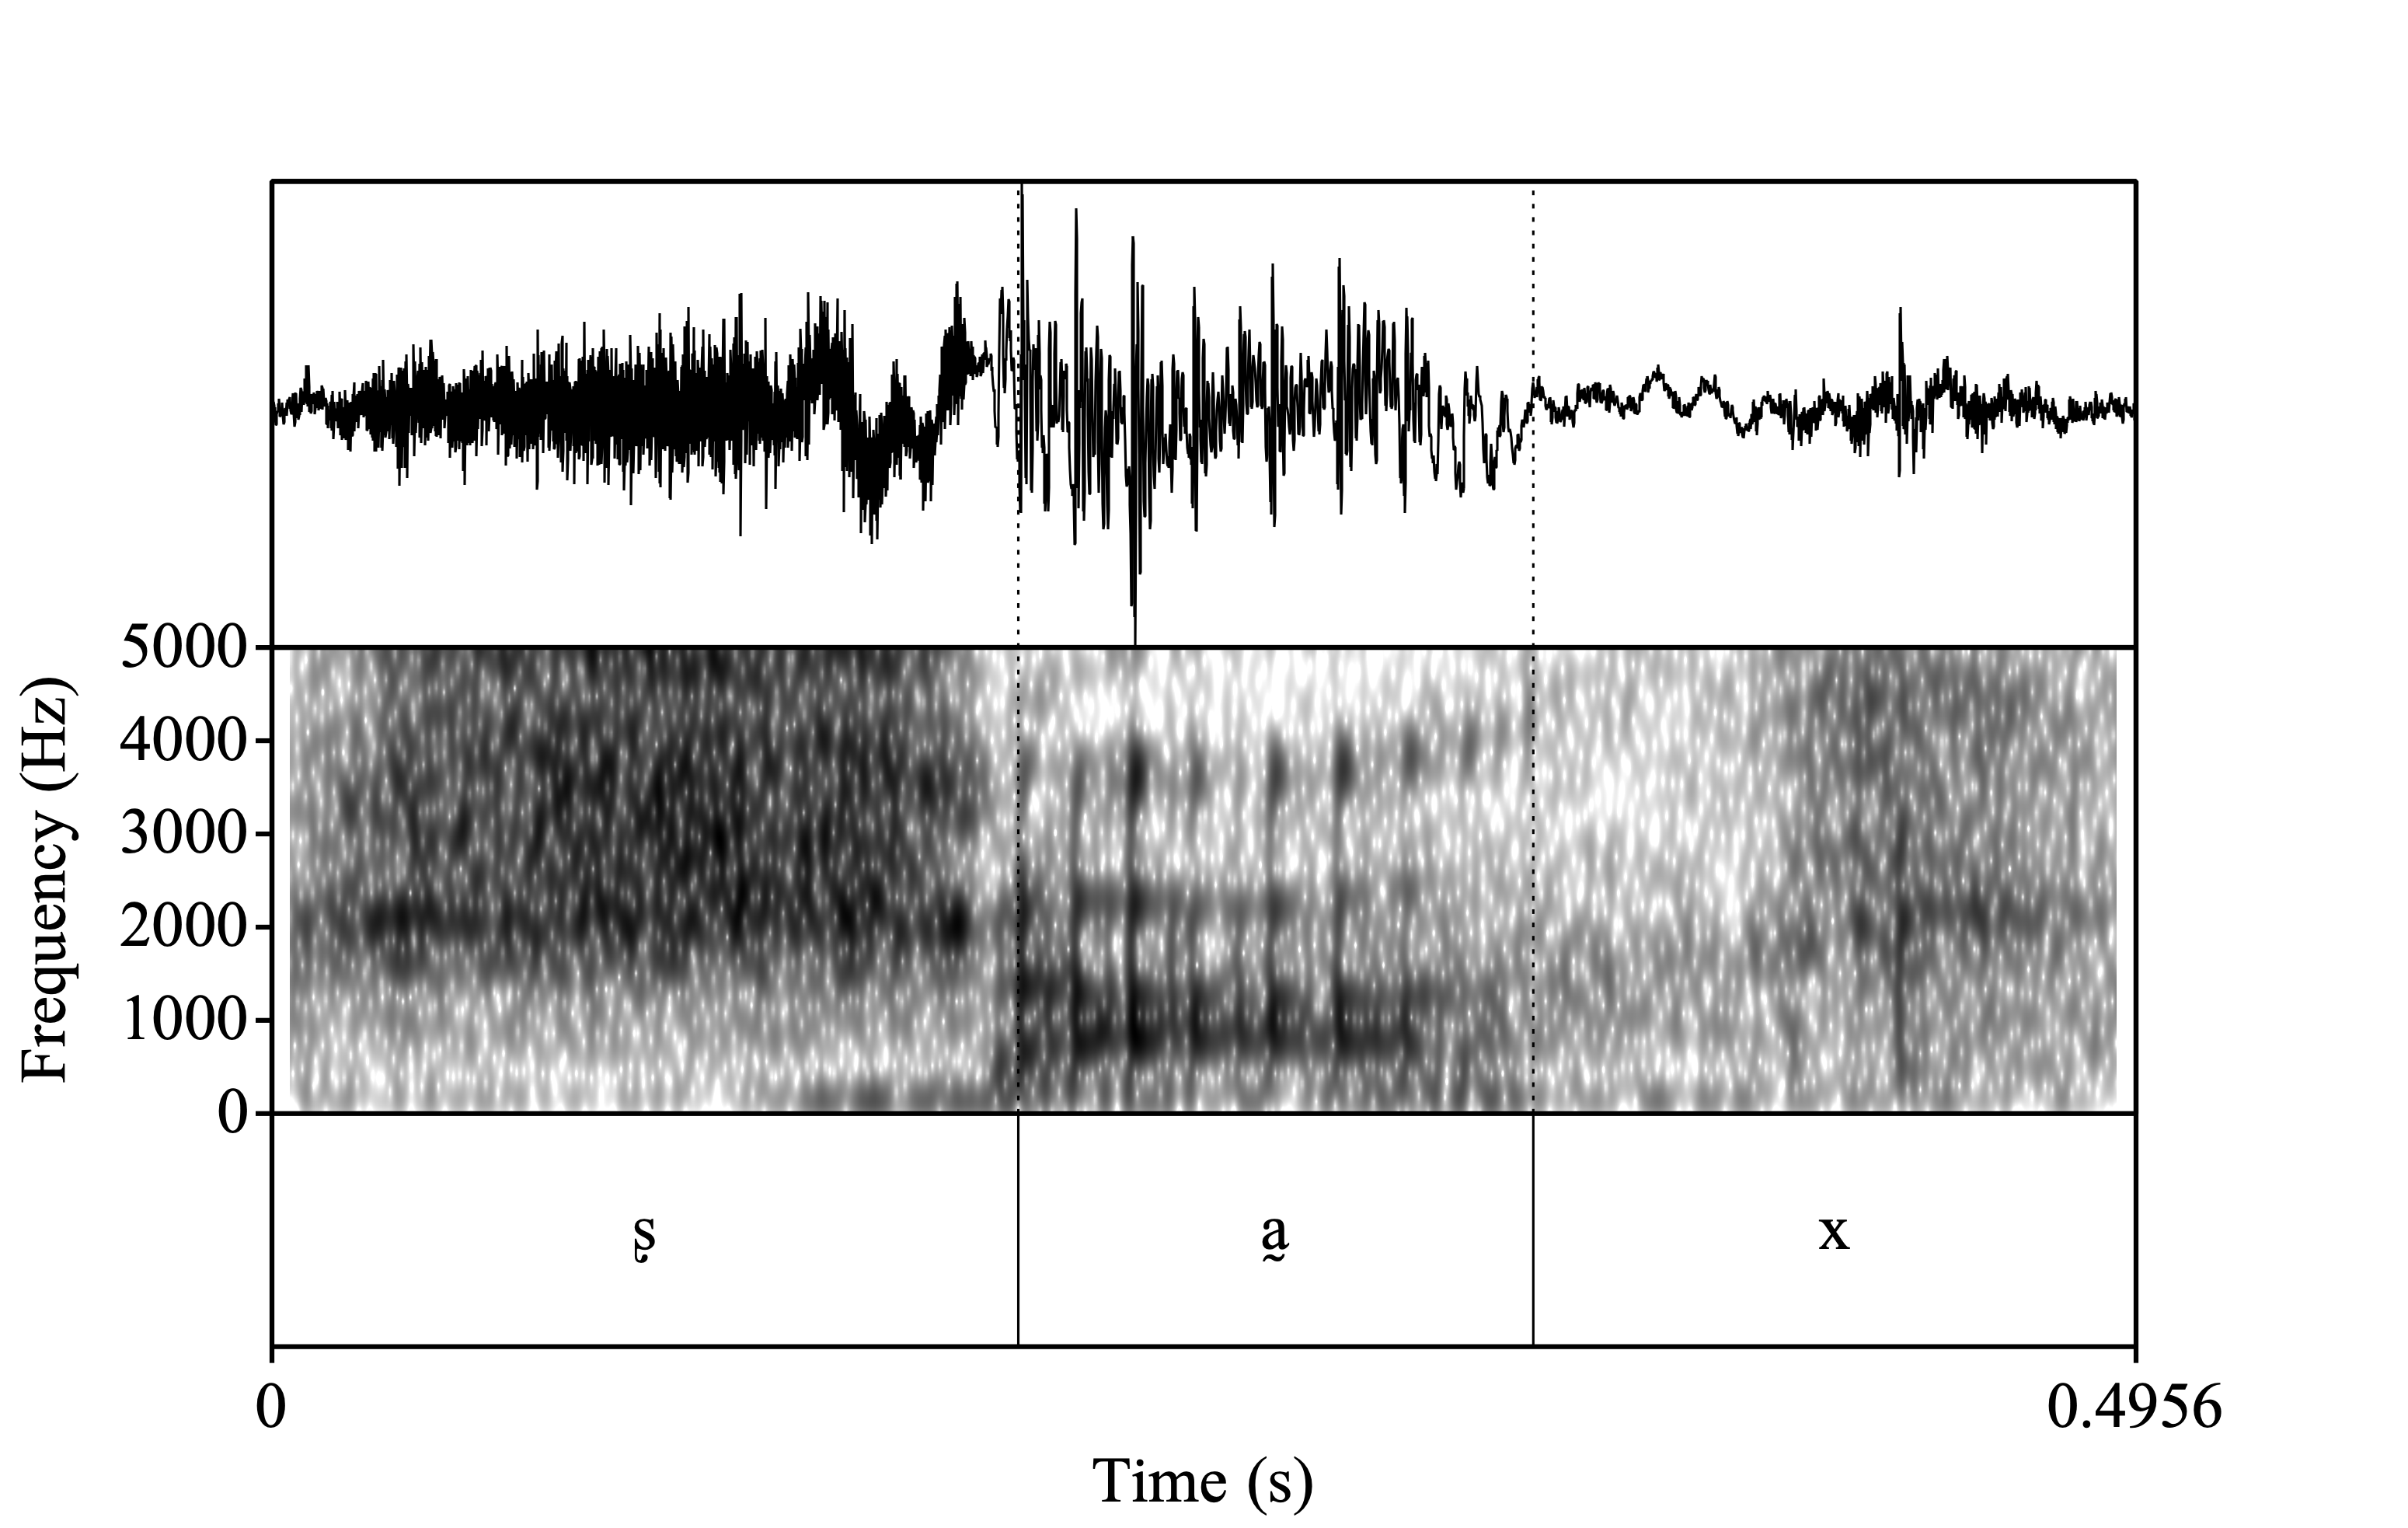
\includegraphics[width=\linewidth]{Images/RD_xa'ag.png}
% 		\caption{\textit{xa'ag} `topil'}
% 		\label{fig:RDxa'ag}
% 	\end{subfigure}
% 	\caption{Comparison of RD's laryngealized vowels in \textit{za'a} `corncob' and \textit{xa'ag} `topil'}
% 	\label{fig:RDLaryngeal}
% \end{figure}

% %------------------------------------
% \subsection{Interaction of Tone and Phonation} \label{sec:Interaction}
% %------------------------------------

% Most previous work on the interaction of tone and phonation has been focused on the languages of East and Southeast Asia (e.g., \cite{masicaDefiningLinguisticArea1976,thurgoodVietnameseTonogenesisRevising2002,yipTone2002,enfieldArealLinguisticsMainland2005,michaudComplexTonesEast2012,brunelleTonePhonationSoutheast2016}). What has been found in these descriptions is that certain tones and phonations are codependent. For example, \citet{smalleyProblemsConsonantsTone1976} and \citet{ratliffMeaningfulToneStudy1992} both describe White Hmong's \textit{-g} tone as being a mid-low tone with breathy phonation, and Mandarin's tone 3 is often associated with creaky phonation \citep{hockettPeipingPhonology1947}. \citet{brunelleTonePerceptionNorthern2009} found that creaky phonation plays an important role in producing certain tones. Additionally, work on S'gaw Karen has found that two tones are only differentiated by some form of non-modal phonation (Boehm p.c.). 

% However, there have been some observations–especially in Mesoamerica–that tone and phonation are independent of each other \citep[e.g.,][]{silvermanLaryngealComplexityOtomanguean1997,garellekAcousticConsequencesPhonation2011}. This means that tone can independently occur with any phonation type. This has also been extensively described in multiple Zapotecan languages \citep[e.g.,][]{,avelinobecerraTopicsYalalagZapotec2004,avelinoAcousticElectroglottographicAnalyses2010, chavez-peonInteractionMetricalStructure2010, campbellZenzontepecChatinoAspect2011,villardPhonologyMorphologyZacatepec2015, lopeznicolasEstudiosFonologiaGramatica2016}

% \citet{chavez-peonInteractionMetricalStructure2010} describes the tone and phonation interactions in San Lucas Quiaviní Zapotec (SLQZ), a central valley variety of Zapotec. The distribution of tone and phonation is found in Table~\ref{tab:SLQZ}. We see that in SLQZ, both low- and falling-tones have the full range of possible combinations. However, we see gaps in the high-tone for breathy and rising tones that can only occur with modal phonation. 

% \begin{table}[!ht]
% 	\centering
% 	\caption{SLQZ tone and phonation interactions \citep{chavez-peonInteractionMetricalStructure2010}.}
% 	\label{tab:SLQZ}
% 	 \begin{tabular}{lcccc}
% 	  \lsptoprule
% 					  &	 \textbf{Modal}  & \textbf{Breathy} & \textbf{Creaky} & \textbf{Interrupted} \\
% 		  High	& ✔︎ & -- & ✔︎ & ✔︎ \\
% 		  Low & ✔︎ & ✔︎ & ✔︎ & ✔︎ \\
% 		  Falling & ✔︎ & ✔︎ & ✔︎ & ✔︎ \\
% 		  Rising & ✔︎ & -- & -- & -- \\
% 	  \lspbottomrule
% 	 \end{tabular}
% \end{table}

Based on elicitation data collected from 2020-2022, SLZ has a more expansive distribution of tone and phonation when compared to SLQZ but seems to be very similar to other Northern Zapotec varieties \citep[e.g.,][]{avelinobecerraTopicsYalalagZapotec2004}. The distribution of SLZ tonal and phonation combinations are given in Table~\ref{tab:ToneVoiceQuality}.
\begin{table}[!h]
	\caption{SLZ tone and voice quality combinations.}
	\label{tab:ToneVoiceQuality}
	\centering

	\begin{tabular}{lcccc}
	\lsptoprule
		& \textbf{Modal} & \textbf{Breathy} & \textbf{Checked} & \textbf{Rearticulated} \\
	\hline
	High		& ✔︎ & -- & ✔︎ & ✔︎ \\
	Mid			& ✔︎ & ✔︎ & ✔︎ & ✔︎ \\
	Low			& ✔︎ & ✔︎ & ✔︎ & ✔︎ \\
	High-Low	& ✔︎ & ✔︎ & ✔︎ & ✔︎ \\
	Mid-High	& ✔︎	& ✔︎ & -- & ✔︎ \\
	\lspbottomrule
	\end{tabular}
\end{table}

% One of the striking things in this is the lack of high tone with breathy phonation. This gap is interesting because of the long-time association of high pitch with breathiness \citep[a good overview–of this association and other phonation types–is found in][]{eslingVoiceQualityLaryngeal2019}. This gap is common across the Zapotecan languages that have breathy voice (Campbell p.c.). Regarding breathy phonation in SLQZ, one of the Valley Zapotec varieties, \citet{uchiharaToneRegistrogenesisQuiavini2016} offers some convincing evidence that the phonation originated in syllables with low tone and then spread to other tones via analogy. Investigating the origin of breathy voice in SLZ would be important in understanding how breathy vowels originated in the Zapotecan family where breathy voice is rare typologically \citep{ariza-garciaPhonationTypesTones2018}. Such a study is beyond the scope of this paper.  